\section{Logistic Regression}

\textbf{Logistic Regression} được lựa chọn là baseline model đầu tiên do tính \textit{đơn giản, hiệu quả và khả năng diễn giải cao}. Model này phù hợp với bài toán phân loại nhị phân tin thật/giả vì:

\begin{itemize}
    \item \textbf{Linear interpretability}: Có thể giải thích tầm quan trọng của từng feature thông qua coefficients
    \item \textbf{Probabilistic output}: Cung cấp confidence score cho predictions
    \item \textbf{Robust với high-dimensional data}: Hoạt động tốt với 25,030 features từ TF-IDF
    \item \textbf{Fast training}: Convergence nhanh với solver liblinear
\end{itemize}

\textbf{Kết quả hiệu suất:}
\begin{itemize}
    \item \textit{Test Accuracy}: 93.80\% - hiệu suất rất tốt
    \item \textit{Training time}: 13.3 phút 
    \item \textit{Precision/Recall}: 0.94 cho cả hai lớp (cân bằng tốt)
    \item \textbf{Nhược điểm}: Overfitting nghiêm trọng (generalization gap = 0.3076)
\end{itemize}

\section{SVC Linear}

\textbf{LinearSVC} được chọn như một alternative robust hơn cho high-dimensional text data. Lý do lựa chọn:

\begin{itemize}
    \item \textbf{Margin maximization}: Tìm decision boundary tối ưu nhất
    \item \textbf{Robust với outliers}: Ít bị ảnh hưởng bởi noise trong text data
    \item \textbf{Memory efficient}: LinearSVC scale tốt hơn RBF SVM với large datasets
    \item \textbf{Regularization}: Built-in regularization giúp giảm overfitting
\end{itemize}

\textbf{Kết quả hiệu suất:}
\begin{itemize}
    \item \textit{Test Accuracy}: 92.53\% - thấp hơn Logistic Regression nhưng vẫn excellent
    \item \textit{Training time}: 4.6 phút - nhanh hơn đáng kể (3x)
    \item \textit{Generalization}: Overfitting measure chỉ 0.0842 (GOOD) - generalize tốt hơn nhiều
    \item \textbf{Trade-off}: Hy sinh chút accuracy để có model stable hơn
\end{itemize}

\section{Hiệu chỉnh siêu tham số với SVC Linear}

Do LinearSVC cho thấy \textbf{khả năng generalization tốt hơn}, chúng tôi thực hiện hyperparameter tuning để tối ưu hóa hiệu suất. Quá trình này bao gồm:

\noindent   \textbf{Grid Search Strategy:}
\begin{itemize}
    \item \textit{Sample-based tuning}: Sử dụng 5,000 mẫu để accelerate search
    \item \textit{3-fold Cross Validation}: Đảm bảo robust evaluation
    \item \textit{336 parameter combinations}: Comprehensive search space
    \item \textit{Parameters tuned}: C, loss, penalty, tolerance, dual, class\_weight
\end{itemize}

\noindent\textbf{Kết quả sau tuning:}
\begin{itemize}
    \item \textit{Cross-validation score}: 92.44\% trên sample data
    \item \textit{Final test accuracy}: 92.62\% - cải thiện nhẹ từ 92.53\%
    \item \textit{Training time}: 281.9 giây (4.7 phút) - vẫn nhanh
    \item \textit{Balanced performance}: Precision/Recall = 0.93 cho cả hai lớp
\end{itemize}

\textbf{So sánh tổng quan:}
\begin{figure}[h!]
\centering
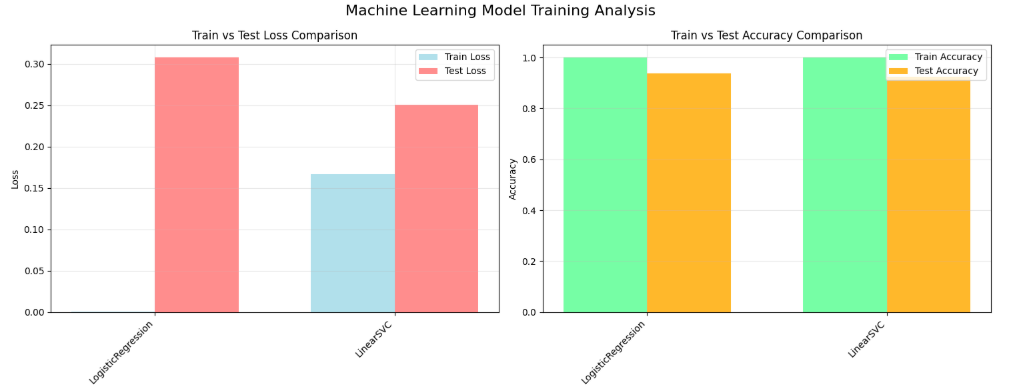
\includegraphics[width=1\textwidth]{images/8.png}
\end{figure}
\FloatBarrier

\noindent Từ visualization results, \textbf{Logistic Regression} đạt accuracy cao nhất (93.80\%) nhưng có \textit{overfitting nghiêm trọng}. \textbf{LinearSVC} (sau tuning) có accuracy thấp hơn chút (92.62\%) nhưng \textit{generalize tốt hơn} và \textit{training nhanh hơn} đáng kể.

\noindent Việc lựa chọn model cuối cùng phụ thuộc vào priority: \textit{highest accuracy} (Logistic Regression) hay \textit{better generalization} (LinearSVC tuned). Trong production environment, LinearSVC có thể reliable hơn do ít overfitting.